% Options for packages loaded elsewhere
\PassOptionsToPackage{unicode}{hyperref}
\PassOptionsToPackage{hyphens}{url}
%
\documentclass[
]{article}
\usepackage{lmodern}
\usepackage{amssymb,amsmath}
\usepackage{ifxetex,ifluatex}
\ifnum 0\ifxetex 1\fi\ifluatex 1\fi=0 % if pdftex
  \usepackage[T1]{fontenc}
  \usepackage[utf8]{inputenc}
  \usepackage{textcomp} % provide euro and other symbols
\else % if luatex or xetex
  \usepackage{unicode-math}
  \defaultfontfeatures{Scale=MatchLowercase}
  \defaultfontfeatures[\rmfamily]{Ligatures=TeX,Scale=1}
\fi
% Use upquote if available, for straight quotes in verbatim environments
\IfFileExists{upquote.sty}{\usepackage{upquote}}{}
\IfFileExists{microtype.sty}{% use microtype if available
  \usepackage[]{microtype}
  \UseMicrotypeSet[protrusion]{basicmath} % disable protrusion for tt fonts
}{}
\usepackage{xcolor}
\IfFileExists{xurl.sty}{\usepackage{xurl}}{} % add URL line breaks if available
\IfFileExists{bookmark.sty}{\usepackage{bookmark}}{\usepackage{hyperref}}
\hypersetup{
  pdftitle={Quechua word structure results},
  pdfauthor={Meg Cychosz},
  hidelinks,
  pdfcreator={LaTeX via pandoc}}
\urlstyle{same} % disable monospaced font for URLs
\usepackage[margin=1in]{geometry}
\usepackage{longtable,booktabs}
% Correct order of tables after \paragraph or \subparagraph
\usepackage{etoolbox}
\makeatletter
\patchcmd\longtable{\par}{\if@noskipsec\mbox{}\fi\par}{}{}
\makeatother
% Allow footnotes in longtable head/foot
\IfFileExists{footnotehyper.sty}{\usepackage{footnotehyper}}{\usepackage{footnote}}
\makesavenoteenv{longtable}
\usepackage{graphicx,grffile}
\makeatletter
\def\maxwidth{\ifdim\Gin@nat@width>\linewidth\linewidth\else\Gin@nat@width\fi}
\def\maxheight{\ifdim\Gin@nat@height>\textheight\textheight\else\Gin@nat@height\fi}
\makeatother
% Scale images if necessary, so that they will not overflow the page
% margins by default, and it is still possible to overwrite the defaults
% using explicit options in \includegraphics[width, height, ...]{}
\setkeys{Gin}{width=\maxwidth,height=\maxheight,keepaspectratio}
% Set default figure placement to htbp
\makeatletter
\def\fps@figure{htbp}
\makeatother
\setlength{\emergencystretch}{3em} % prevent overfull lines
\providecommand{\tightlist}{%
  \setlength{\itemsep}{0pt}\setlength{\parskip}{0pt}}
\setcounter{secnumdepth}{5}
\usepackage{booktabs}
\usepackage{longtable}
\usepackage{array}
\usepackage{multirow}
\usepackage{wrapfig}
\usepackage{float}
\usepackage{colortbl}
\usepackage{pdflscape}
\usepackage{tabu}
\usepackage{threeparttable}
\usepackage{threeparttablex}
\usepackage[normalem]{ulem}
\usepackage{makecell}
\usepackage{xcolor}

\title{Quechua word structure results}
\author{Meg Cychosz}
\date{8/11/2020}

\begin{document}
\maketitle

{
\setcounter{tocdepth}{2}
\tableofcontents
}
\hypertarget{results}{%
\section{Results}\label{results}}

The primary research objective of this study is to measure the speech production patterns of child and adult Quechua speakers between and within morphemes. Results begin with descriptive statistics concerning the amount of coarticulation and VC sequence duration by age group and morphological environment (within versus between morphemes). Then, a series of models are fit to predict coarticulation and duration by age and morphological environment. These models are complemented by an analysis highlighting how coarticulation interacts with duration differently in adults and children in the two morphological environments.

All analyses were conducted in the RStudio computing environment (version: 1.3.1056; rstudio, 2020). Data visualizations were created with \texttt{ggplot2} (Wickham, 2016). Modeling was conducted using the \texttt{lme4} (Bates et al., 2015), \texttt{lmerTest} (Kuznetsova et al., 2017), and \texttt{glmmTMB} (Brooks et al., 2017) packages and summaries were presented with \texttt{papaja} (Aust \& Barth, 2019) and \texttt{Stargazer} (Hlavac, 2018). Tests of residual normality were conducted using the \texttt{normtest} package (Gavrilov \& Pusev, 2014). The significance of potential model parameters was determined using a combination of log-likelihood comparisons between models, AIC estimations, and p-values procured from model summaries. In all models, continuous predictors were mean-centered to facilitate model interpretation.

\hypertarget{modeling-interaction-of-coarticulation-and-duration}{%
\subsection{Modeling interaction of coarticulation and duration}\label{modeling-interaction-of-coarticulation-and-duration}}

\hypertarget{coarticulation}{%
\subsubsection{Coarticulation}\label{coarticulation}}

The degree of coarticulation between the VC sequences {[}ap{]} and {[}am{]} was measured using the spectral distance metric described in the Methods. For this metric, coarticulation is quantified as the Euclidean distance between the spectral vectors of two adjacent phones, henceforth the Mel spectral distance. A larger spectral distance between phones equates to \emph{less} coarticulation between the phones.

\begin{table}

\caption{\label{tab:ap-coartic-tbl}Mean spectral distance between [a] and [p] by age and word position}
\centering
\begin{tabular}[t]{lrrrr}
\toprule
\multicolumn{1}{c}{ } & \multicolumn{2}{c}{Across boundary} & \multicolumn{2}{c}{Within boundary} \\
\cmidrule(l{3pt}r{3pt}){2-3} \cmidrule(l{3pt}r{3pt}){4-5}
Age & Spectral\_Distance  & SD  & Spectral\_Distance & SD\\
\midrule
5 & 17.42 & 4.64 & 19.63 & 4.56\\
6 & 17.62 & 4.70 & 19.78 & 4.59\\
7 & 17.04 & 4.68 & 19.18 & 5.90\\
8 & 18.50 & 6.03 & 21.35 & 6.76\\
9 & 16.21 & 7.02 & 17.51 & 7.79\\
\addlinespace
10 & 14.92 & 5.09 & 15.93 & 5.07\\
adult & 14.99 & 3.64 & 14.51 & 3.03\\
\bottomrule
\end{tabular}
\end{table}

\begin{table}

\caption{\label{tab:am-coartic-tbl}Mean spectral distance between [a] and [m] by age and word position}
\centering
\begin{tabular}[t]{lrrrr}
\toprule
\multicolumn{1}{c}{ } & \multicolumn{2}{c}{Across boundary} & \multicolumn{2}{c}{Within boundary} \\
\cmidrule(l{3pt}r{3pt}){2-3} \cmidrule(l{3pt}r{3pt}){4-5}
Age & Spectral\_Distance  & SD  & Spectral\_Distance & SD\\
\midrule
5 & 7.94 & 3.13 & 8.71 & 3.39\\
6 & 8.44 & 3.08 & 9.54 & 4.76\\
7 & 8.43 & 3.11 & 8.86 & 3.80\\
8 & 9.89 & 3.99 & 9.73 & 3.78\\
9 & 7.43 & 2.64 & 8.06 & 3.11\\
\addlinespace
10 & 8.21 & 3.43 & 8.30 & 4.25\\
adult & 7.44 & 4.19 & 7.00 & 3.34\\
\bottomrule
\end{tabular}
\end{table}

Table \ref{tab:ap-coartic-tbl} shows the mean Mel spectral distance between the segments in {[}ap{]} (words inflected with \emph{-pi} for the across morpheme boundary condition) and Table \ref{tab:am-coartic-tbl} shows this for {[}am{]} (words inflected with \emph{-man} for the across morpheme boundary condition). Unsurprisingly, there is a larger average spectral distance between the vowel and plosive in {[}ap{]} than the vowel and nasal in {[}am{]} because the segments in {[}am{]} have increased acoustic similarity (sonority, voicing). Next, looking by age group for coarticulation between {[}ap{]} shows that the amount of coarticulation between segments increases as children age. This is likely due to the increased speaking rate in the older cohorts and adults, as will become apparent when these results are crossed with sequence duration. There is also a large amount of between-child variability, even within age group (see Appendices I for by-speaker plots). For example, the eight-year-old children appear to have the largest spectral distance between {[}a{]} and {[}p{]}, but the group SD is also highest.

There is less within-group variability in {[}ap{]} productions in the adult speakers (reflected in the adults' smaller SD of the mean). Furthermore, variability does not appear to decrease linearly as both the nine and ten-year-old cohorts exhibit larger SDs than the five and six-year-olds. However, this could also reflect the smaller sample sizes in the older cohorts (5 ten-year-olds and 5 nine-year-olds but 10 each in the five- and six-year-old cohorts).

For the coarticulation patterns between segments in {[}am{]}, adults and children coarticulate similarly, irrespective of age group. There is slightly greater variability in the amount of coarticulation (larger SD) in the adult group.

\hypertarget{duration}{%
\subsubsection{Duration}\label{duration}}

The following descriptive statistics outline the interaction of coarticulation and sequence duration. Duration interacts with coarticulation, and age, as speakers coarticulate more in fast speech (Gay, 1981), and adults speak faster than children (Lee et al., 1999).

\begin{table}

\caption{\label{tab:ap-dur-tbl}Mean duration of [ap] sequence by age and word position}
\centering
\begin{tabular}[t]{lrrrr}
\toprule
\multicolumn{1}{c}{ } & \multicolumn{2}{c}{Across boundary} & \multicolumn{2}{c}{Within boundary} \\
\cmidrule(l{3pt}r{3pt}){2-3} \cmidrule(l{3pt}r{3pt}){4-5}
Age & Duration (ms) & SD  & Duration (ms) & SD\\
\midrule
5 & 228.7 & 47 & 339.9 & 52\\
6 & 242.5 & 45 & 334.4 & 59\\
7 & 245.1 & 57 & 319.8 & 60\\
8 & 226.9 & 56 & 329.3 & 43\\
9 & 216.6 & 36 & 312.6 & 56\\
\addlinespace
10 & 212.8 & 50 & 302.3 & 63\\
adult & 205.7 & 47 & 197.0 & 59\\
\bottomrule
\end{tabular}
\end{table}

\begin{table}

\caption{\label{tab:am-dur-tbl}Mean duration of [am] sequence by age and word position}
\centering
\begin{tabular}[t]{lrrrr}
\toprule
\multicolumn{1}{c}{ } & \multicolumn{2}{c}{Across boundary} & \multicolumn{2}{c}{Within boundary} \\
\cmidrule(l{3pt}r{3pt}){2-3} \cmidrule(l{3pt}r{3pt}){4-5}
Age & Duration (ms) & SD  & Duration (ms) & SD\\
\midrule
5 & 214.4 & 45 & 251.2 & 66\\
6 & 217.9 & 58 & 247.8 & 62\\
7 & 209.8 & 42 & 244.6 & 60\\
8 & 218.2 & 63 & 247.1 & 53\\
9 & 199.8 & 30 & 231.8 & 64\\
\addlinespace
10 & 194.3 & 33 & 239.9 & 57\\
adult & 175.6 & 36 & 173.7 & 39\\
\bottomrule
\end{tabular}
\end{table}

Table \ref{tab:ap-dur-tbl} maps average sequence duration of {[}ap{]} by age and word position and Table \ref{tab:am-dur-tbl} does so for {[}am{]}. Duration of {[}ap{]} decreases with age, with adult speakers exhibiting the shortest average {[}ap{]} duration for both word positions. The average duration of {[}ap{]} sequences within morphemes tended to be longer than the duration of {[}ap{]} sequences across boundaries for all of the children. This pattern was reversed in the adult speakers whose average {[}ap{]} duration within morpheme boundaries was actually \emph{shorter} than across. The patterns by morphological environment will be revisited in the following section of the Results.

Turning to the sequence {[}am{]}, the average duration of {[}am{]} in adult speakers was shorter than all of the children; and like {[}ap{]}, {[}am{]} duration also decreases with age, across and within morphemes.

Concerning differences by word position, all child age groups showed, on average, shorter {[}am{]} durations in the across morpheme condition, contrary to the finding that {[}ap{]} sequence duration was longer in the across morpheme condition for adults. However, the average duration of {[}am{]} by word position in adults only differed by approximately 2 ms while the average within morpheme condition in children was approximately 30 ms greater than the across morpheme condition. Thus, for both {[}am{]} and {[}ap{]} sequences, there appears to be a difference in sequence duration by word position for adult and child speakers. In the following section we turn to the modeling of coarticulation before illustrating how degree of coarticulation interacts with duration differently in the adults and children.

\hypertarget{modeling}{%
\subsubsection{Modeling}\label{modeling}}

A series of generalized linear mixed effect models (GLMMs) were fit to predict degree of coarticulation (Mel spectral distance between each V and C). GLMMs were chosen instead of the more common linear mixed effect models due to the non-normality of the residual \textbf{VC Sequence duration} (henceforth simply \textbf{Sequence Duration}) which was included in all models.\footnote{Shapiro tests of kurtosis and skewness for \textbf{Sequence duration} indicated that we could reject the null hypothesis that the residual's distribution did not differ significantly from a normal distribution. Kurtosis t=5.53, p\textless.001 and skewness: t=1.07, p\textless.001 (Shapiro et al., 1968).} Specifically, the response variable \textbf{Spectral distance} and the residual \textbf{Sequence duration} are both limited to non-negative values (as all VC sequences had some distance between the V and C and all had a duration), with a resultant right skew to the data distribution.

The choice to fit gamma GLMMs, as opposed to log-normalizing \textbf{Sequence duration} and fitting linear mixed models, reflects some recent suggestions in cognitive psychology to avoid data transformation, even for commonly-transformed variables such as time, duration, or response time, to facilitate between-study comparison (Liceralde, 2018; Lo \& Andrews, 2015). However, there is not yet a consensus in the literature on the use of transformed versus untransformed variables. Consequently, gamma GLMMs were fit using a log linking function to appropriately model the skewed, non-Gaussian distribution of the residual. Then, in a supplementary analysis, all modeling procedures were replicated with linear mixed effects models that included a transformed \textbf{Sequence duration} variable. Final model results were broadly consistent across the two modeling approaches; see Supplementary analysis for details.

Baseline GLMMs included random slopes of \textbf{Participant} by \textbf{Word}. Model building then began in a forward-testing manner with predictors added in the following order: \textbf{Syllable Count} (fit with weighted effect coding for all models), \textbf{Sequence duration}, \textbf{VC sequence} ({[}ap{]} or {[}am{]}), \textbf{Age} (adult or child), \textbf{Environment} ({[}within morpheme or between morphemes{]}), and interactions. \textbf{Syllable Count} was included in the modeling in an attempt to isolate the effect of \textbf{Environment} on speech production from prosodic structure since within-morpheme stimulus items tended to be shorter than across-morpheme items (see Methods).\footnote{To further ensure that the difference by \textbf{Environment} was due to morphological structure, all models were additionally fit with the covariate \textbf{Word Duration} (in ms), instead of \textbf{Syllable Count} (models were not fit with both since \textbf{Word Duration} and \textbf{Syllable Count} are highly correlated). Results were broadly the same: the three-way interaction of \textbf{Sequence duration}, \textbf{VC sequence}, and \textbf{Environment} improved upon model fits controlling for \textbf{Word Duration} with the same direction of the effect. Like the models that control for prosodic structure with the covariate, \textbf{Syllable Count}, these models also suggest that the speech production differences by word environment were more likely morphological, not prosodic, in nature.}

The best model fit included \textbf{Syllable Count} and the four-variable interaction of \textbf{Sequence duration}, \textbf{VC sequence}, \textbf{Age}, and \textbf{Environment}. This four-variable interaction indicates that the relationship between coarticulation and duration differs between adults and children. Given the difficulty in interpreting four-variable interactions, separate models were fit for adults and children to facilitate coefficient interpretation. The summary for the model containing adults and children together is included in Appendix E.

Best model fit for the adult and child models included \textbf{Syllable Count} and the three-variable interaction of \textbf{Sequence duration}, \textbf{VC sequence}, and \textbf{Environment}: the improvement of models with this interaction over models with the four independent effects was significant for the adult model at alpha level \textless.05 (\(\chi\)\textsuperscript{2} = 11.18, df=9,13 p=.02) and the child model (\(\chi\)\textsuperscript{2} = 36.52, df=9,13, p\textless.001). The final adult model summary is listed in Table \ref{tab:adult-model-sum} and the child model summary is listed in Table \ref{tab:child-model-sum}.\footnote{In the model summaries for the children and adults, the coefficients and standard error measurements were multiplied by 100 to make the otherwise small coefficients more interpretable. This step does not effect the direction or magnitude of the effect between predictors and outcome variables.}

For the child model, the addition of the variable \textbf{Age Group} (levels: 5, 6, 7, 8, 9, 10; fit with weighted effect coding) improved upon a model with \textbf{Syllable Count} and the interaction of \textbf{Sequence duration}, \textbf{VC sequence}, and \textbf{Environment}. The direction of the effect of \textbf{Age Group} indicates that the child participants tended to coarticulate more with age, just as the adults studied coarticulated more than the children, likely because the older children and adults spoke faster.

\begin{table}[tbp]

\begin{center}
\begin{threeparttable}

\caption{\label{tab:adult-model-sum}Model predicting coarticulation in adults}

\begin{tabular}{llllll}
\toprule
term & \multicolumn{1}{c}{estimate} & \multicolumn{1}{c}{S.E.} & \multicolumn{1}{c}{z.statistic} & \multicolumn{1}{c}{p.value} & \multicolumn{1}{c}{95\% CI}\\
\midrule
Intercept & 203.64 & 5.33 & 38.20 & 0.00 & 2.14,1.93\\
Syllable count:2 & 10.45 & 4.42 & 2.36 & 0.02 & 0.19,0.02\\
Syllable count:3 & -4.32 & 1.75 & -2.47 & 0.01 & -0.01,-0.08\\
Syllable count:4 & 6.27 & 2.80 & 2.24 & 0.03 & 0.12,0.01\\
Sequence duration & 0.36 & 0.06 & 6.45 & 0.00 & 0,0\\
Environment:across morpheme & 6.97 & 7.21 & 0.97 & 0.33 & 0.21,-0.07\\
VC sequence:ap & 60.66 & 6.32 & 9.59 & 0.00 & 0.73,0.48\\
Sequence duration*Environment:across morpheme & -0.17 & 0.08 & -2.18 & 0.03 & 0,0\\
Sequence duration*VC sequence:ap & -0.22 & 0.07 & -3.26 & 0.00 & 0,0\\
Environment:across morpheme*VC sequence:ap & 8.66 & 7.74 & 1.12 & 0.26 & 0.24,-0.07\\
Sequence duration*Environment:across morpheme*VC sequence:ap & 0.25 & 0.09 & 2.72 & 0.01 & 0,0\\
\bottomrule
\end{tabular}

\end{threeparttable}
\end{center}

\end{table}

\begin{table}[tbp]

\begin{center}
\begin{threeparttable}

\caption{\label{tab:child-model-sum}Model predicting coarticulation in children}

\begin{tabular}{llllll}
\toprule
term & \multicolumn{1}{c}{estimate} & \multicolumn{1}{c}{S.E.} & \multicolumn{1}{c}{z.statistic} & \multicolumn{1}{c}{p.value} & \multicolumn{1}{c}{95\% CI}\\
\midrule
Intercept & 212.26 & 1.75 & 121.63 & 0.00 & 2.16,2.09\\
Syllable count:2 & 5.77 & 2.40 & 2.40 & 0.02 & 0.1,0.01\\
Syllable count:3 & -1.52 & 1.18 & -1.28 & 0.20 & 0.01,-0.04\\
Syllable count:4 & -1.07 & 1.58 & -0.68 & 0.50 & 0.02,-0.04\\
Sequence duration & 0.09 & 0.02 & 4.15 & 0.00 & 0,0\\
Environment:across morpheme & 2.94 & 2.77 & 1.06 & 0.29 & 0.08,-0.02\\
VC sequence:ap & 71.30 & 3.33 & 21.39 & 0.00 & 0.78,0.65\\
Age:10 & -9.24 & 1.75 & -5.29 & 0.00 & -0.06,-0.13\\
Age:6 & 3.00 & 1.20 & 2.49 & 0.01 & 0.05,0.01\\
Age:7 & 0.57 & 1.03 & 0.56 & 0.58 & 0.03,-0.01\\
Age:8 & 9.99 & 1.38 & 7.24 & 0.00 & 0.13,0.07\\
Age:9 & -10.39 & 1.80 & -5.79 & 0.00 & -0.07,-0.14\\
Sequence duration*Environment:across morpheme & 0.00 & 0.03 & -0.09 & 0.93 & 0,0\\
Sequence duration*VC sequence:ap & -0.04 & 0.03 & -1.38 & 0.17 & 0,0\\
Environment:across morpheme*VC sequence:ap & -1.67 & 3.67 & -0.45 & 0.65 & 0.06,-0.09\\
Sequence duration*Environment:across morpheme*VC sequence:ap & -0.10 & 0.04 & -2.34 & 0.02 & 0,0\\
\bottomrule
\end{tabular}

\end{threeparttable}
\end{center}

\end{table}

In the adult and child models, a positive coefficient for the predictor \textbf{VC sequence}, with the reference level `{[}am{]}', shows that there was greater spectral distance between the segments in {[}ap{]} than {[}am{]}, as we would anticipate given the acoustic signatures of {[}m{]} (voiced, sonorant) versus {[}p{]} (voiceless, transient) (adult model: \(\beta\)=60.66, z=9.59, p\textless.001; child model: \(\beta\)=71.3, z=21.39, p\textless.001).

A positive coefficient for \textbf{Sequence duration} indicates that longer duration VC sequences tend to be less coarticulated (greater spectral distance between phones) (child model: \(\beta\)=0.09, z=4.15, p\textless.001; adult model: \(\beta\)=0.36, z=6.45, p\textless.001). The coefficients suggest that when speakers, both adults and children alike, speak slower, they tend to coarticulate less. There is, however, an interaction between several of these predictors, which will demonstrate that children in particular do not always coarticulate less in longer-duration sequences. The direction of the interaction between \textbf{Sequence duration}, \textbf{VC sequence}, and \textbf{Environment} differs between the adult and child speakers so this will be interpreted separately for the two groups in the following section.

Finally, the parameter \textbf{Syllable Count} was significant for the adult and child models, though the effect differed by group. Children tended to coarticulate progressively more in longer words. Adults coarticulated differently by word size, but coarticulation did not increase in longer words. These unanticipated age differences will be explored in the following section of the results.

~
~

\begin{figure}
\centering
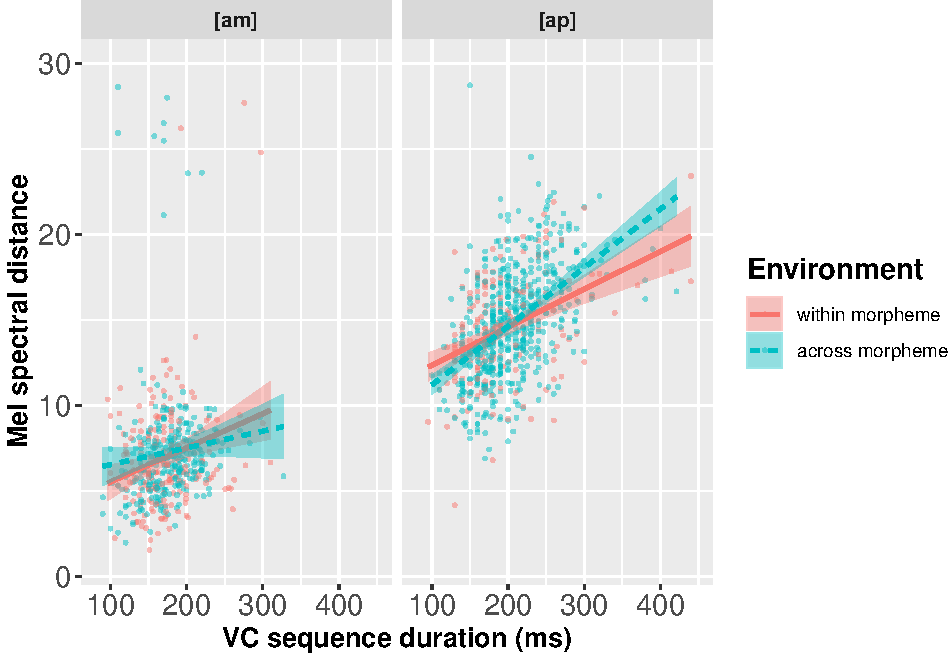
\includegraphics{3_ch3_results_files/figure-latex/adult-int-plot-1.pdf}
\caption{\label{fig:adult-int-plot}Coarticulation within VC sequence by sequence duration and morphological environment in adult speakers}
\end{figure}

\begin{figure}
\centering
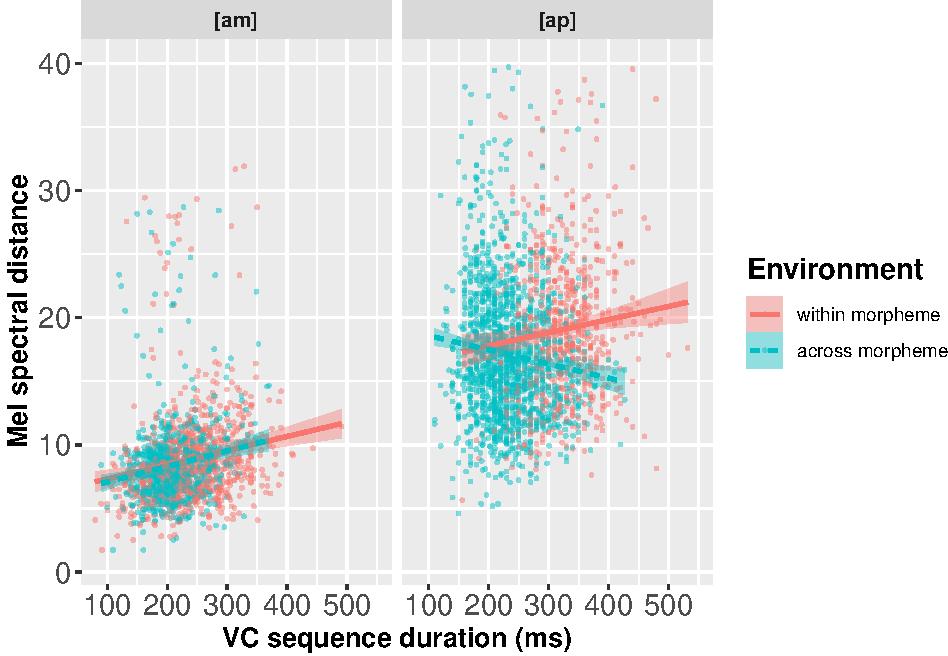
\includegraphics{3_ch3_results_files/figure-latex/child-int-plot-1.pdf}
\caption{\label{fig:child-int-plot}Coarticulation within VC sequence by sequence duration and morphological environment in all child speakers}
\end{figure}

\hypertarget{adults}{%
\paragraph{Adults}\label{adults}}

For the adult model, the interaction between \textbf{Sequence duration}, \textbf{VC sequence}, and \textbf{Environment} suggests a difference in the relationship between the response variable---amount of coarticulation---and \textbf{Sequence duration} that differs by \textbf{Environment} and \textbf{VC sequence}. As Figure \ref{fig:adult-int-plot} demonstrates, this difference by \textbf{Environment} is apparent in the steepness of the slope for the `across morpheme' and `within morpheme' conditions for {[}am{]} and {[}ap{]}. To quantify this difference for the sequence {[}am{]}, the slopes of the two conditions were calculated. As the {[}am{]} panel in Figure \ref{fig:adult-int-plot} suggests, the slope for the `within morpheme' condition was steeper (2.14) than the slope for the `across morpheme' condition (2.06),\footnote{To reflect the data visualizations, these slopes were calculated on the beta coefficients before the coefficients were scaled by 100.} suggesting a different relationship between duration and coarticulation between the two word environments in adults.

Overall, the significance of the interaction \textbf{Sequence duration}, \textbf{VC sequence}, and \textbf{Environment} in adult speakers shows two important results: first, adults distinguish by word environment, both for {[}ap{]} versus {[}a\#p{]} sequences and {[}am{]} versus {[}a\#m{]} sequences. Second, complicating this finding, is the fact that adults distinguish between word environments differently depending upon the VC sequence. For {[}ap{]}, though adults coarticulate roughly equally across and within morphemes, the relationship between duration and coarticulation (longer duration equates to less coarticulation) is stronger in the `across morpheme' condition. For {[}am{]}, adults also distinguish between the two morphological environments by the relationship of VC duration and coarticulatory degree, but the effect of condition is reversed: the relationship between duration and coarticulation is stronger for the `within morpheme' condition.

Thus, returning to one of the central research questions - does adult coarticulation differ by word environment - we find that adults do coarticulate differently in the two word environments. Despite the differences by word environment, there was still a positive relationship between duration and amount of coarticulation for all combinations of VC sequences and word environments. Adults consistently coarticulate less in longer-duration sequences. This result suggests that adult speakers may have one overarching articulatory plan for all environments and both VC sequences measured. The following section demonstrates how this relationship between duration and coarticulation may not be uniform between adults and children.

\hypertarget{children}{%
\paragraph{Children}\label{children}}

In the child model, the significant interaction of \textbf{Sequence duration}, \textbf{VC sequence}, and \textbf{Environment} suggests that children do not coarticulate similarly in longer-duration sequences for all combinations of \textbf{Environment} and \textbf{VC sequence} (Figure \ref{fig:child-int-plot}). Specifically, for {[}ap{]} sequences that occur across morpheme boundaries, the negative slope indicates that children actually coarticulate \emph{more} in longer duration sequences. The positive slope for the within morpheme boundary condition suggests that children coarticulate less in longer-duration sequences, in line with all of the adult patterns. So, children coarticulate more between segments at morpheme boundaries in words inflected with the locative marker \emph{-pi} than between those same segments that occur within morphemes.

\begin{figure}
\centering
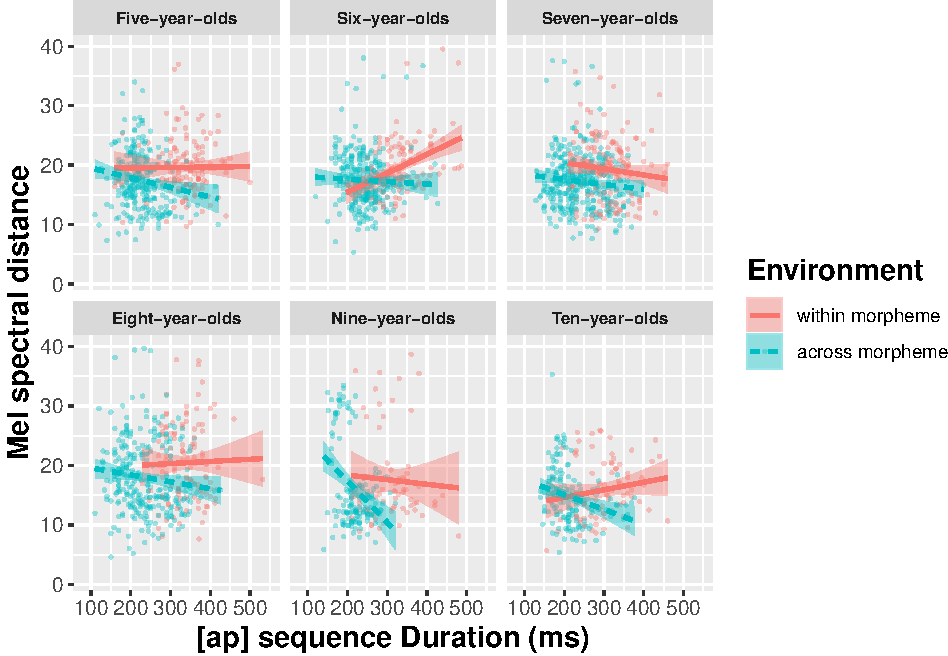
\includegraphics{3_ch3_results_files/figure-latex/child-facet-ap-1.pdf}
\caption{\label{fig:child-facet-ap}Coarticulation within {[}ap{]} by sequence duration, morphological environment, and age in child speakers}
\end{figure}

This negative relationship between duration and spectral distance is counter to the positive relationship for every combination of VC sequence and word environment in adult speakers. Adults consistently coarticulate less in longer-duration sequences regardless of environment or VC sequence. The facet plot in Figure \ref{fig:child-facet-ap} plots this relationship between duration and coarticulation for {[}ap{]} for each age group (5-10 years) to ensure a consistent pattern. All age groups show the same negative relationship: the longer the {[}ap{]} sequence, the more the children coarticulate between {[}a{]} and {[}p{]} in the across morpheme condition.

\begin{figure}
\centering
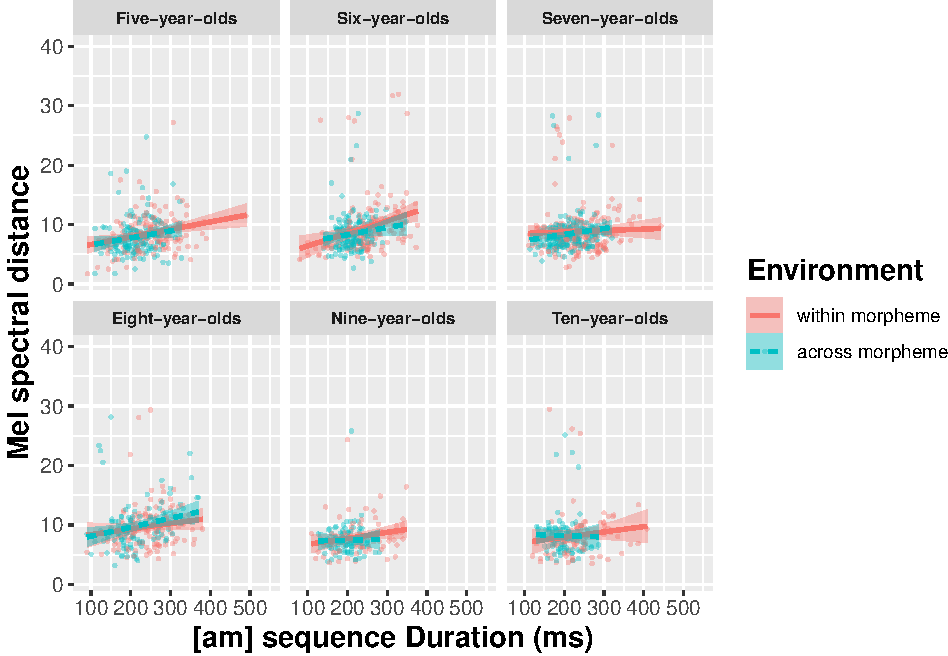
\includegraphics{3_ch3_results_files/figure-latex/child-facet-am-1.pdf}
\caption{\label{fig:child-facet-am}Coarticulation within {[}am{]} by sequence duration, morphological environment, and age in child speakers}
\end{figure}

The results for {[}am{]} in children demonstrate broadly similar results to the adult speakers: children coarticulate less between segments in longer-duration {[}am{]} sequences. The facet plot in Figure \ref{fig:child-facet-am} once again shows a similar effect for each age group. Given the between-subject variability that typically characterizes child speech, these patterns by environment are further broken apart by individual child for each age group (age 5-10) (Appendix I) to ensure no large outliers with regards to the patterning by word environment. The results by are broadly similar across speakers.

In sum, modeling results suggest that morphological structure is reflected in the speech of adults and children. However, the structure manifests in different ways between the two groups. Adults have a single plan for both environments, and even both VC sequences: adults coarticulate less in longer-duration sequences. For the most part, children show a similar duration-coarticulation relationship. The stark difference between adults and children emerges in the {[}ap{]} sequence patterning. Children differentiate between morphological environments via the relationship between duration and coarticulation as they coarticulate more in longer-duration sequences across morpheme boundaries and coarticulate \emph{less} in longer-duration sequences within morphemes. For words inflected with \emph{-man}, children show a similar pattern to adults, though children do not differentiate by environment coarticulatorily. Rather, across morpheme sequences are shorter in duration than within morpheme sequences for the children.

~
~

\hypertarget{compensatory-shortening}{%
\subsection{Compensatory shortening}\label{compensatory-shortening}}

One finding that emerged from the modeling in the previous section was a different effect of word length on coarticulation between the adults and children. The degree of children's coarticulation tended to progressively increase in words with more syllables; no such pattern was apparent for the adults.

An exploratory analysis was conducted to explain the different relationship between coarticulation and word length for adults and children. This analysis asks, does the direction of the relationship between word length and coarticulation also hold for duration? Since coarticulation and duration are negatively correlated, this analysis predicts that duration would decrease as a function of the number of syllables in a word for the children. As such, the children's productions would reflect the phenomenon of \textsc{Compensatory Shortening} (also known as polysyllabic shortening), or the tendency for segment durations to shorten in longer-duration and/or polysyllabic words (Harrington et al., 2015; Lehiste 1972; Munhall et al., 1992).

An effect of word length upon duration was predicted for the adults as well. However, just as it was found that coarticulation did not increase as a function of word length in the adult model, it is anticipated that adults likewise will not compensate durationally for longer words. As a result, the children, but not the adults, would exhibit compensatory shortening during their word production.

\begin{figure}
\centering
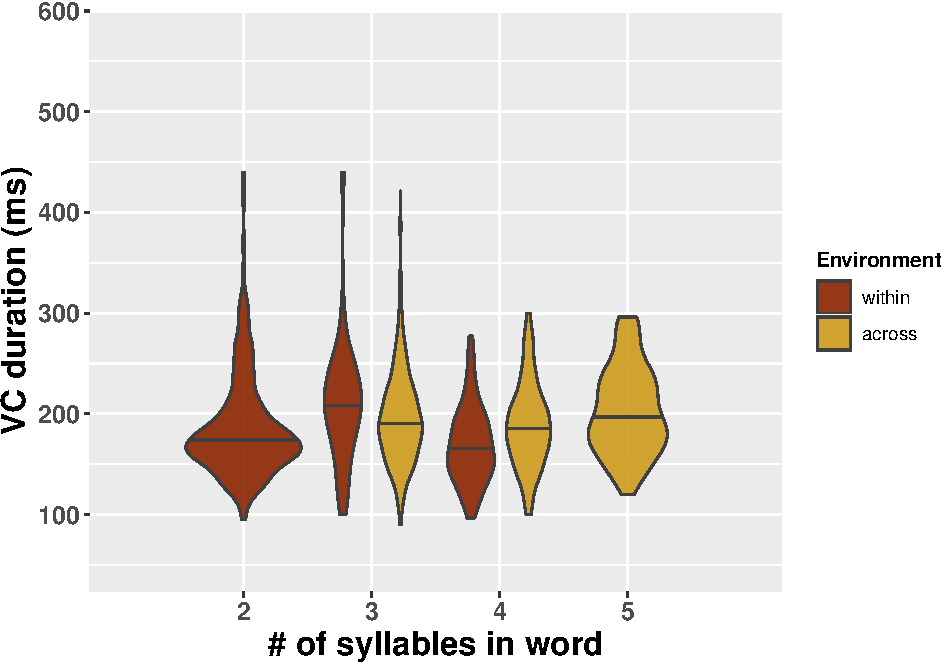
\includegraphics{3_ch3_results_files/figure-latex/compshort-adults-1.pdf}
\caption{\label{fig:compshort-adults}Sequence duration by word length and word environment: Adults}
\end{figure}

\begin{table}[!htbp] \centering 
  \caption{Model predicting VC duration: children} 
  \label{} 
\begin{tabular}{@{\extracolsep{5pt}}lc} 
\\[-1.8ex]\hline 
\hline \\[-1.8ex] 
 Intercept & 230.96$^{***}$ \\ 
  & (228.03, 233.88) \\ 
  & \\ 
 Age:6 & 8.66$^{***}$ \\ 
  & (4.74, 12.58) \\ 
  & \\ 
 Age:7 & 3.78$^{*}$ \\ 
  & (0.43, 7.12) \\ 
  & \\ 
 Age:8 & 0.25 \\ 
  & ($-$4.26, 4.76) \\ 
  & \\ 
 Age:9 & $-$14.46$^{***}$ \\ 
  & ($-$20.31, $-$8.61) \\ 
  & \\ 
 Age:10 & $-$17.23$^{***}$ \\ 
  & ($-$22.92, $-$11.54) \\ 
  & \\ 
 VC sequence:[ap] & 28.31$^{***}$ \\ 
  & (24.38, 32.23) \\ 
  & \\ 
 Two syllables & 57.70$^{***}$ \\ 
  & (54.37, 61.03) \\ 
  & \\ 
 Three syllables & $-$21.63$^{***}$ \\ 
  & ($-$23.54, $-$19.72) \\ 
  & \\ 
 Four syllables & $-$33.27$^{***}$ \\ 
  & ($-$37.97, $-$28.56) \\ 
  & \\ 
\hline \\[-1.8ex] 
Observations & 3,877 \\ 
Log Likelihood & $-$20,476.84 \\ 
Akaike Inf. Crit. & 40,977.68 \\ 
Bayesian Inf. Crit. & 41,052.84 \\ 
\hline 
\hline \\[-1.8ex] 
\textit{Note:}  & \multicolumn{1}{r}{$^{*}$p$<$0.05; $^{**}$p$<$0.01; $^{***}$p$<$0.001} \\ 
\end{tabular} 
\end{table}

\begin{table}[!htbp] \centering 
  \caption{Model predicting VC duration: adults} 
  \label{} 
\begin{tabular}{@{\extracolsep{5pt}}lc} 
\\[-1.8ex]\hline 
\hline \\[-1.8ex] 
 Intercept & 174.41$^{***}$ \\ 
  & (169.18, 179.63) \\ 
  & \\ 
 VC sequence:[ap] & 29.66$^{***}$ \\ 
  & (22.49, 36.83) \\ 
  & \\ 
 Two syllables & $-$6.12 \\ 
  & ($-$13.46, 1.23) \\ 
  & \\ 
 Three syllables & 4.24$^{*}$ \\ 
  & (0.78, 7.70) \\ 
  & \\ 
 Four syllables & $-$5.36 \\ 
  & ($-$12.97, 2.25) \\ 
  & \\ 
\hline \\[-1.8ex] 
Observations & 1,200 \\ 
Log Likelihood & $-$6,133.52 \\ 
Akaike Inf. Crit. & 12,281.04 \\ 
Bayesian Inf. Crit. & 12,316.67 \\ 
\hline 
\hline \\[-1.8ex] 
\textit{Note:}  & \multicolumn{1}{r}{$^{*}$p$<$0.05; $^{**}$p$<$0.01; $^{***}$p$<$0.001} \\ 
\end{tabular} 
\end{table}

To test the effect of word length (in syllables) upon duration, two linear mixed effects models (adult and child) were fit to predict VC sequence duration (no skewed or non-negative predictors were included in the modeling so GLMMs were not necessary). Model fitting occurred as before in a forward-testing manner: the base model contained random slopes of individual \textbf{Speaker} by \textbf{Word}. Then, parameters were added in the following order: \textbf{Age Group} (fit with weighted effect coding; only included in the child model), \textbf{VC sequence}, \textbf{Number of Syllables} (2-5), and \textbf{Environment} (across versus within). Only the predictors \textbf{Number of Syllables}, \textbf{Age Group}, and \textbf{VC sequence} improved baseline model fit (see Table XXX for the child model summary and Table XXX for the adult model summary; see Appendices G and H for tables with descriptive statistics of duration by age and number of syllables).

In both model summaries, the positive beta coefficients for VC sequence indicate that the {[}ap{]} sequence was significantly longer than the {[}am{]} sequence (as previous models demonstrated). The insignificance of \textbf{Environment} suggests that that the relationship between duration and word length is independent of word environment. The patterns by child age again demonstrate how older children speak faster than younger. Negative coefficients for the nine- and ten-year old children indicate that those children's VC sequences were approximately 14 ms and 17 ms shorter, respectively, than the weighted age group mean.

The primary parameter of interest is \textbf{Syllable Count}. In the child model, the positive coefficient for `2 syllable' stimuli indicates that VC sequence duration in two syllable words was approximately 58 ms longer than the weighted mean word length. The negative coefficients for the `3 syllable' (\(\beta\)=-21.63), `4 syllable' (\(\beta\)=-33.27) and `5 syllable' (\(\beta\)=-28.62; not presented in model summary) stimuli indicate that VC sequences tend to become shorter in longer words. The diverse stimuli in the two- and three-syllable conditions in particular (many different word types) suggest that this relationship by word length is relatively robust for the children.\footnote{The only exception to the tendency to shorten sequences in larger words was that {[}ap{]} sequences are slightly longer in duration in 5-syllable words than 4-syllable words. However, in this exploratory analysis, the differences between the four and five syllable words were not tightly controlled: there were only two different five-syllable word stimuli: \emph{hatun mama-man} `grandmother-\textsc{all}'' and \emph{hatun mama-pi} `grandmother-\textsc{loc}'. We can only speculate that this relationship between sequence duration and number of syllables is strictly linear and would generalize to additional words with more syllables for the children.}

For the adult model, a model with \textbf{Syllable Count} only marginally improved over one without (\(\chi\)\textsuperscript{2} = 6.72, df=4,7, p=.08). Furthermore, only one level of \textbf{Syllable Count}, the three syllable stimuli, significantly predicted sequence duration. This result suggests that 1) word length was not strongly predictive of sequence duration in the adults and 2) adults did not compensate for word length by shortening syllable durations in longer words.

In sum, children appear to compensate for word length in their speech production via coarticulation and duration. Word length is also reflected in the adults' speech patterns, but not in any linear direction that suggests compensatory shortening. Causes behind these age differences are proposed in the Discussion.

\hypertarget{appendices}{%
\section{Appendices}\label{appendices}}

\hypertarget{appendix-e}{%
\subsection{Appendix E}\label{appendix-e}}

\begin{table}[tbp]

\begin{center}
\begin{threeparttable}

\caption{\label{tab:adult-child model sum}Model predicting coarticulation in children 
 and adults}

\begin{tabular}{llllll}
\toprule
term & \multicolumn{1}{c}{estimate} & \multicolumn{1}{c}{S.E.} & \multicolumn{1}{c}{z.statistic} & \multicolumn{1}{c}{p.value} & \multicolumn{1}{c}{95\% CI}\\
\midrule
Intercept & 204.61 & 4.67 & 43.86 & 0.00 & 2.14,1.95\\
Syllable count:2 & 9.48 & 2.05 & 4.62 & 0.00 & 0.13,0.05\\
Syllable count:3 & -3.31 & 0.95 & -3.47 & 0.00 & -0.01,-0.05\\
Syllable count:4 & -1.12 & 1.36 & -0.82 & 0.41 & 0.02,-0.04\\
Sequence duration & 0.29 & 0.06 & 4.99 & 0.00 & 0,0\\
VC sequence:ap & 61.68 & 5.31 & 11.62 & 0.00 & 0.72,0.51\\
Age:child & 6.07 & 4.75 & 1.28 & 0.20 & 0.15,-0.03\\
Environment:across morpheme & 5.73 & 6.35 & 0.90 & 0.37 & 0.18,-0.07\\
Sequence duration*VC sequence:ap & -0.15 & 0.07 & -2.18 & 0.03 & 0,0\\
Sequence duration*Age:child & -0.21 & 0.06 & -3.39 & 0.00 & 0,0\\
VC sequence:ap*Age:child & 6.83 & 6.10 & 1.12 & 0.26 & 0.19,-0.05\\
Sequence duration*Environment:across morpheme & -0.11 & 0.08 & -1.31 & 0.19 & 0,0\\
VC sequence:ap*Environment:across morpheme & 9.12 & 6.95 & 1.31 & 0.19 & 0.23,-0.05\\
Age:child*Environment:across morpheme & 0.42 & 6.30 & 0.07 & 0.95 & 0.13,-0.12\\
Sequence duration*VC sequence:ap*Age:child & 0.13 & 0.08 & 1.68 & 0.09 & 0,0\\
Sequence duration*VC sequence:ap*Environment:across morpheme & 0.16 & 0.09 & 1.69 & 0.09 & 0,0\\
Sequence duration*Age:child*Environment:across morpheme & 0.13 & 0.09 & 1.56 & 0.12 & 0,0\\
VC sequence:ap*Age:child*Environment:across morpheme & -8.35 & 7.69 & -1.09 & 0.28 & 0.07,-0.23\\
Sequence duration*VC sequence:ap*Age:child*Environment:across morpheme & -0.28 & 0.10 & -2.75 & 0.01 & 0,0\\
\bottomrule
\end{tabular}

\end{threeparttable}
\end{center}

\end{table}

\hypertarget{appendix-f}{%
\subsection{Appendix F}\label{appendix-f}}

\begin{figure}
\centering
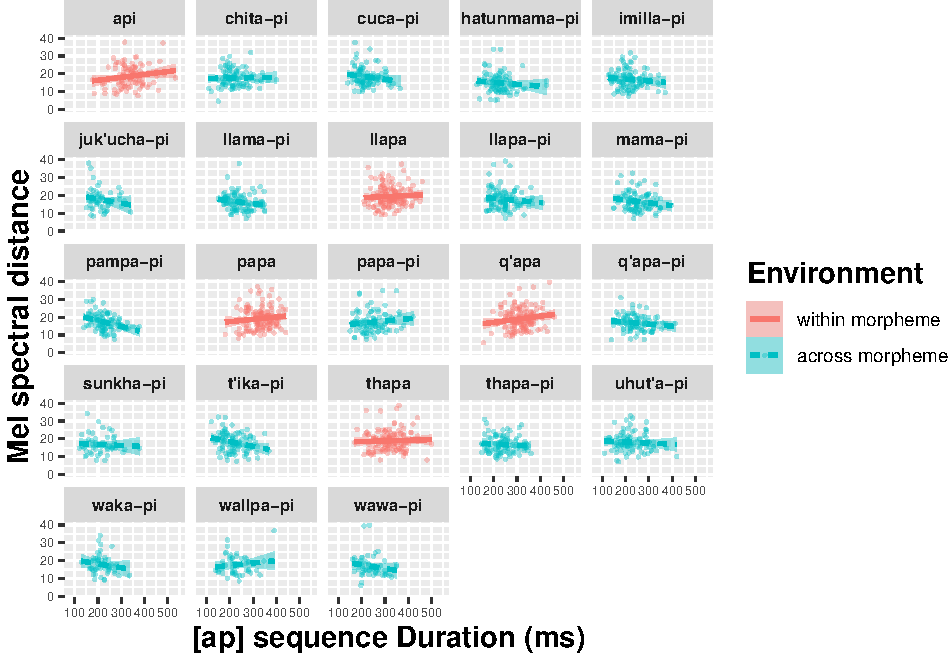
\includegraphics{3_ch3_results_files/figure-latex/child-facet-ap-word-1.pdf}
\caption{\label{fig:child-facet-ap-word}Coarticulation within {[}ap{]} by sequence duration, morphological environment, and word in child speakers}
\end{figure}

\hypertarget{appendix-g}{%
\subsection{Appendix G}\label{appendix-g}}

\begin{table}

\caption{\label{tab:dur-by-syll-kids}Mean VC sequence duration by number of syllables in word for children}
\centering
\begin{tabular}[t]{lrrrr}
\toprule
\multicolumn{1}{c}{ } & \multicolumn{2}{c}{[am]} & \multicolumn{2}{c}{[ap]} \\
\cmidrule(l{3pt}r{3pt}){2-3} \cmidrule(l{3pt}r{3pt}){4-5}
Syllables & Duration (ms) & SD  & Duration (ms) & SD\\
\midrule
2 & 272.9 & 52 & 325.3 & 57\\
3 & 211.6 & 51 & 235.2 & 51\\
4 & 207.6 & 46 & 220.7 & 51\\
5 & 204.1 & 35 & 230.4 & 51\\
\bottomrule
\end{tabular}
\end{table}

\hypertarget{appendix-h}{%
\subsection{Appendix H}\label{appendix-h}}

\begin{table}

\caption{\label{tab:dur-by-syll-adults}Mean VC sequence duration by number of syllables in word for adults}
\centering
\begin{tabular}[t]{lrrrr}
\toprule
\multicolumn{1}{c}{ } & \multicolumn{2}{c}{[am]} & \multicolumn{2}{c}{[ap]} \\
\cmidrule(l{3pt}r{3pt}){2-3} \cmidrule(l{3pt}r{3pt}){4-5}
Syllables & Duration (ms) & SD  & Duration (ms) & SD\\
\midrule
2 & 177.6 & 39 & 192.4 & 57\\
3 & 176.5 & 35 & 210.0 & 50\\
4 & 168.0 & 36 & 195.3 & 43\\
5 & 178.5 & 51 & 207.3 & 40\\
\bottomrule
\end{tabular}
\end{table}

\hypertarget{appendix-i}{%
\subsection{Appendix I}\label{appendix-i}}

\begin{figure}
\centering
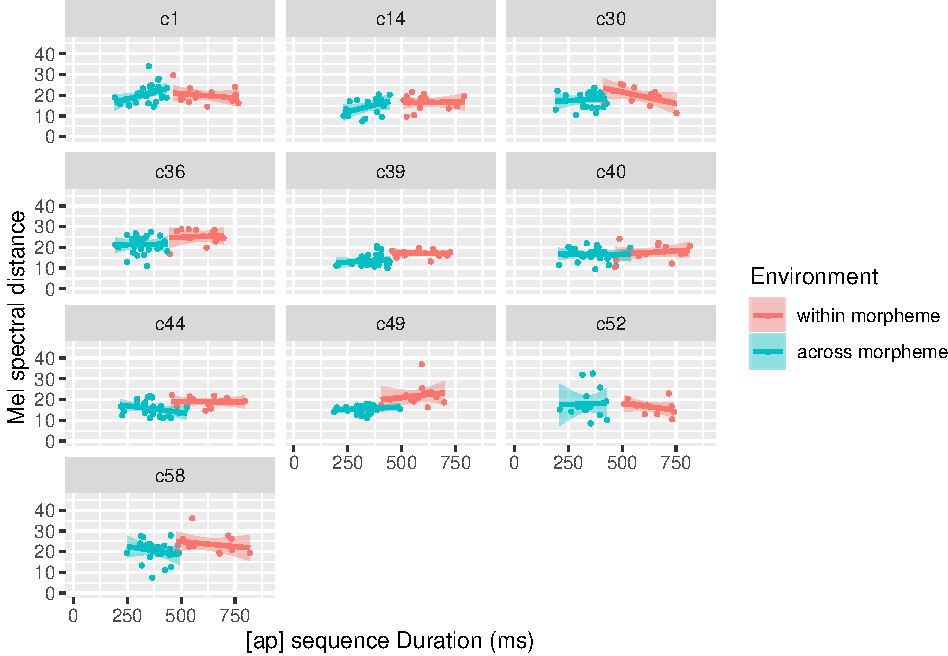
\includegraphics{3_ch3_results_files/figure-latex/five-facet-ap-1.pdf}
\caption{\label{fig:five-facet-ap}Coarticulation by {[}ap{]} duration, word, and morphological environment in five-year-old children}
\end{figure}

\begin{figure}
\centering
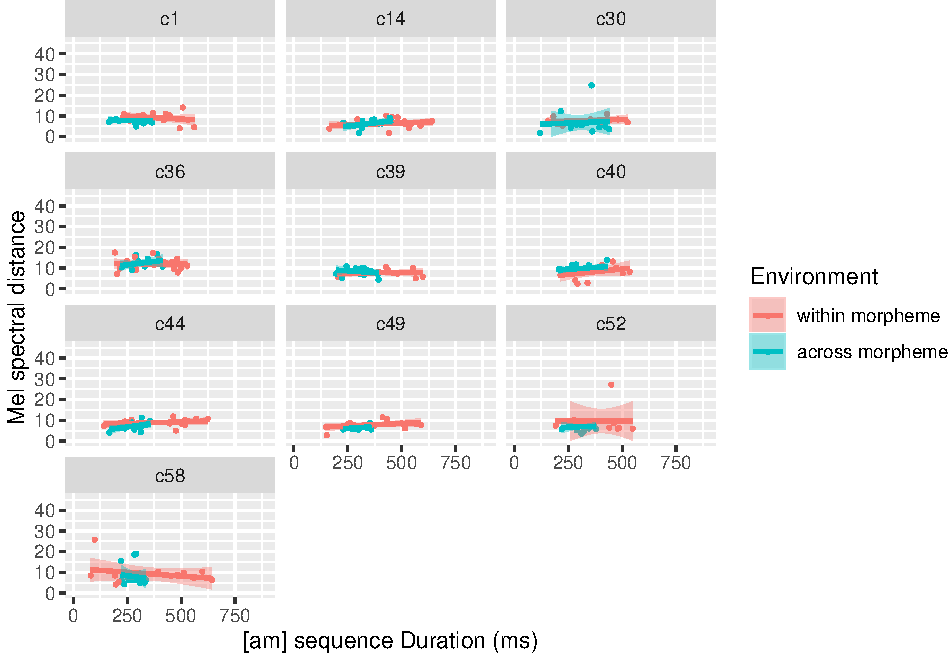
\includegraphics{3_ch3_results_files/figure-latex/five-facet-am-1.pdf}
\caption{\label{fig:five-facet-am}Coarticulation by {[}am{]} duration, word, and morphological environment in five-year-old children}
\end{figure}

\begin{figure}
\centering
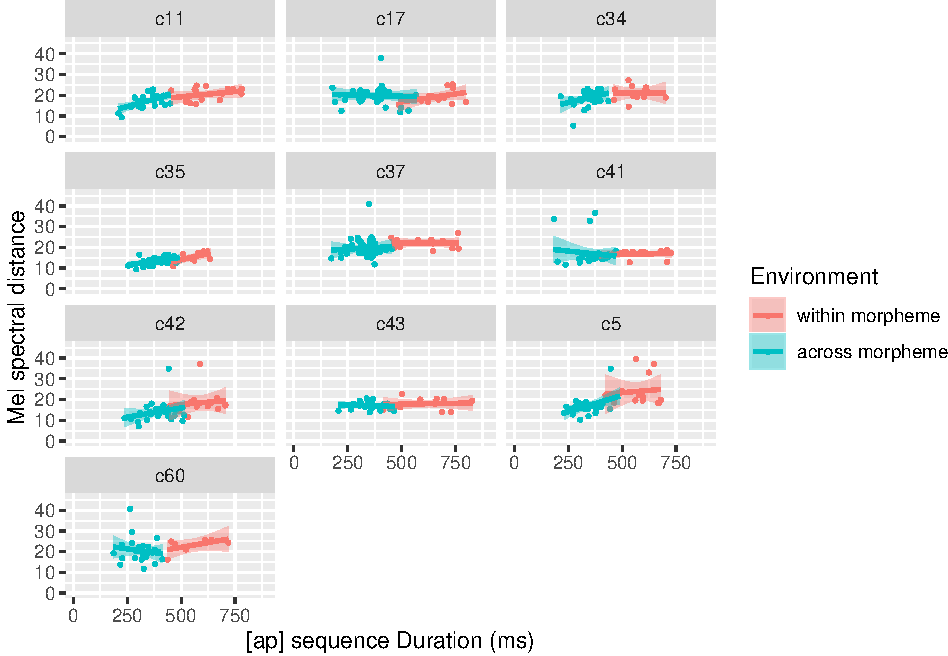
\includegraphics{3_ch3_results_files/figure-latex/six-facet-ap-1.pdf}
\caption{\label{fig:six-facet-ap}Coarticulation by {[}ap{]} duration, word, and morphological environment in six-year-old children}
\end{figure}

\begin{figure}
\centering
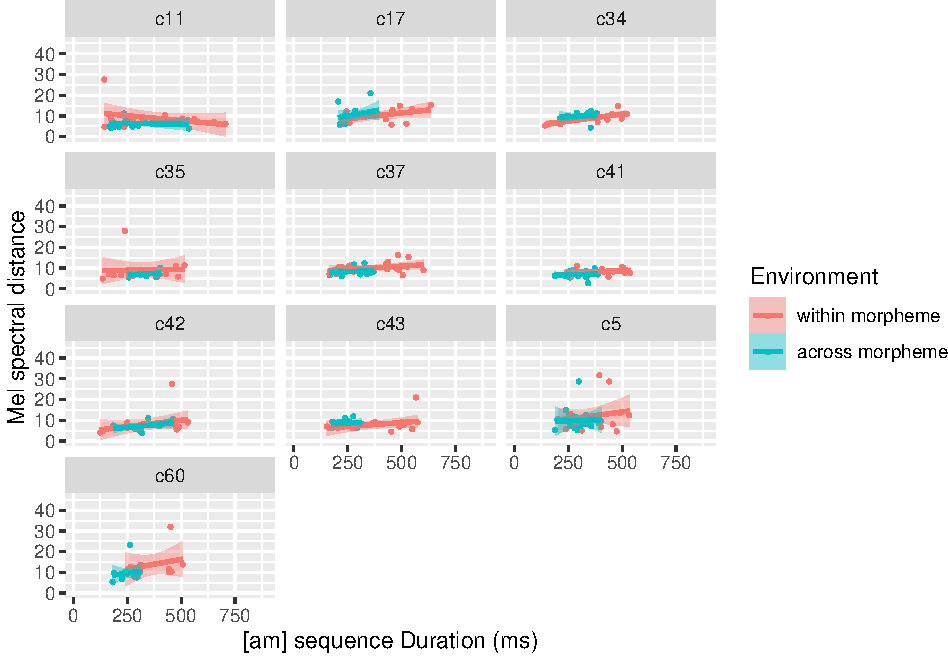
\includegraphics{3_ch3_results_files/figure-latex/six-facet-am-1.pdf}
\caption{\label{fig:six-facet-am}Coarticulation by {[}am{]} duration, word, and morphological environment in six-year-old children}
\end{figure}

\begin{figure}
\centering
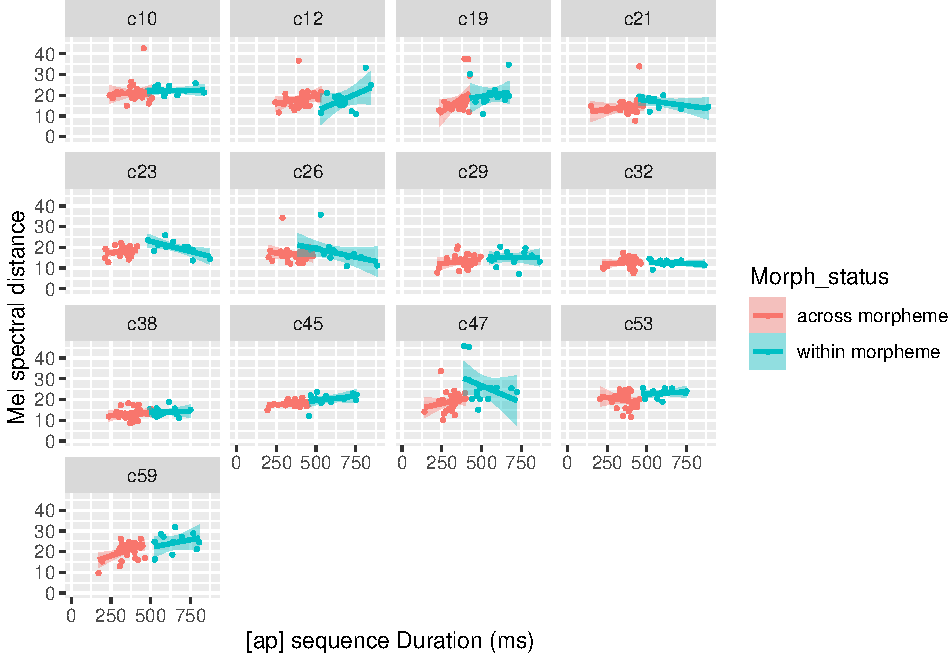
\includegraphics{3_ch3_results_files/figure-latex/seven-facet-ap-1.pdf}
\caption{\label{fig:seven-facet-ap}Coarticulation by {[}ap{]} duration, word, and morphological environment in seven-year-old children}
\end{figure}

\begin{figure}
\centering
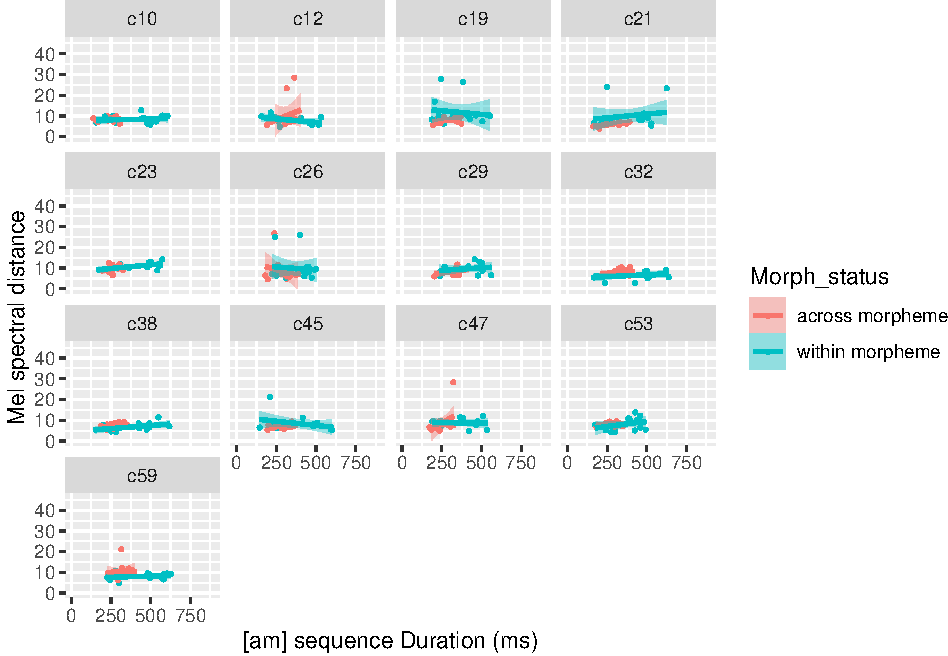
\includegraphics{3_ch3_results_files/figure-latex/seven-facet-am-1.pdf}
\caption{\label{fig:seven-facet-am}Coarticulation by {[}am{]} duration, word, and morphological environment in seven-year-old children}
\end{figure}

\begin{figure}
\centering
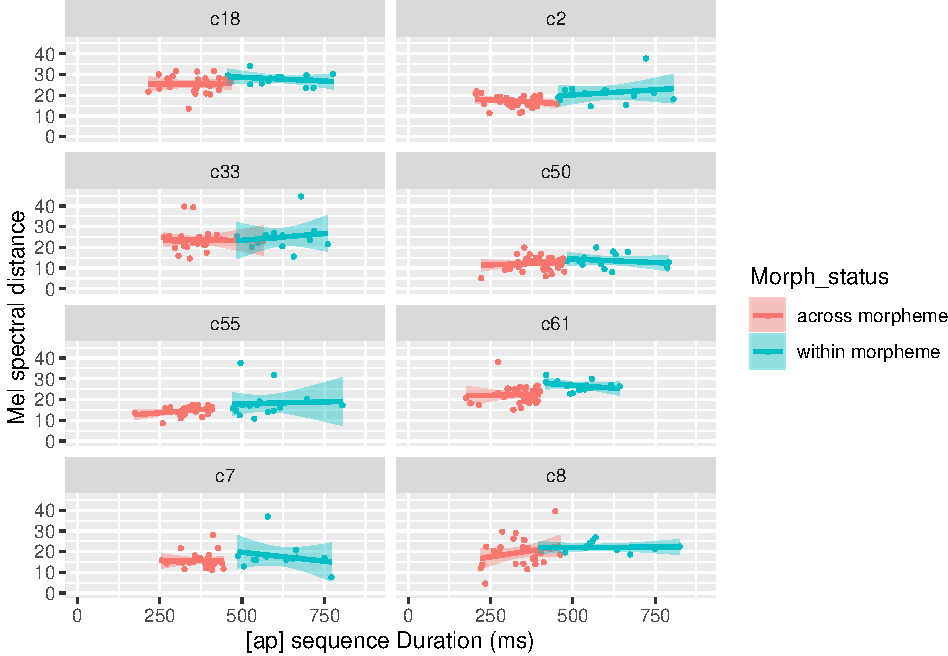
\includegraphics{3_ch3_results_files/figure-latex/eight-facet-ap-1.pdf}
\caption{\label{fig:eight-facet-ap}Coarticulation by {[}ap{]} duration, word, and morphological environment in eight-year-old children}
\end{figure}

\begin{figure}
\centering
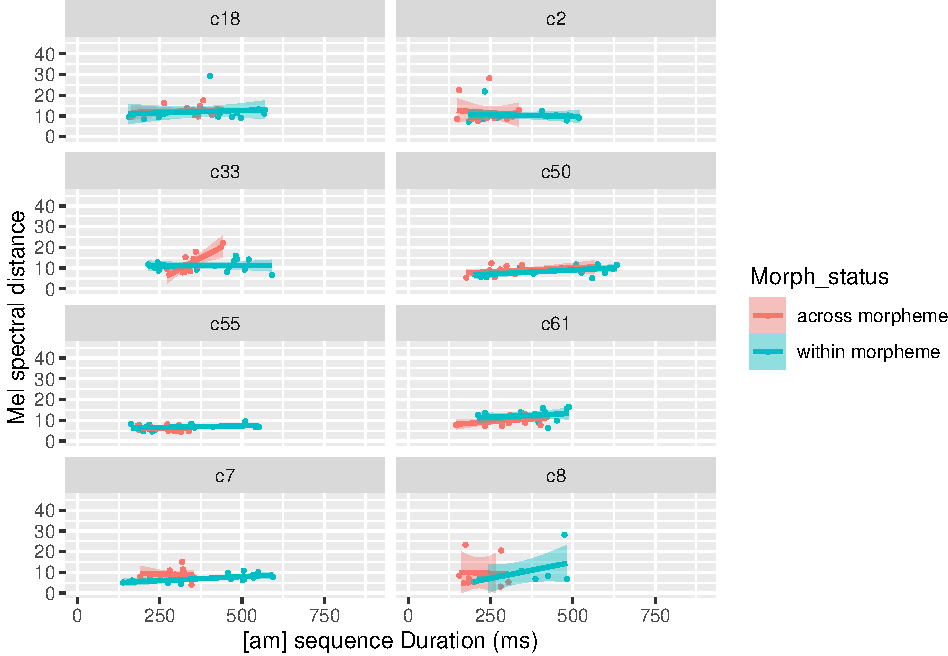
\includegraphics{3_ch3_results_files/figure-latex/eight-facet-am-1.pdf}
\caption{\label{fig:eight-facet-am}Coarticulation by {[}am{]} duration, word, and morphological environment in eight-year-old children}
\end{figure}

\begin{figure}
\centering
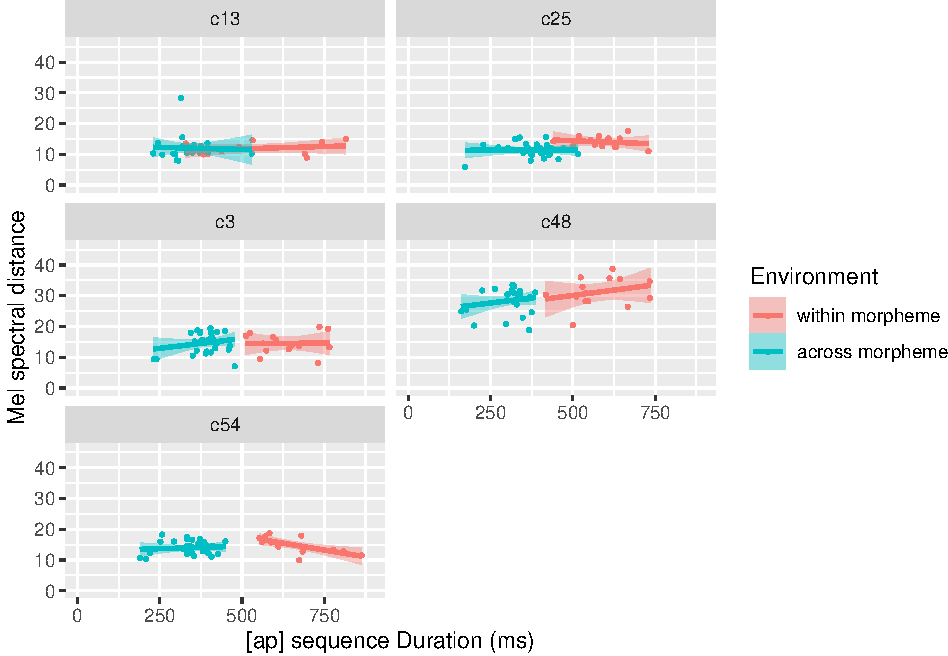
\includegraphics{3_ch3_results_files/figure-latex/nine-facet-ap-1.pdf}
\caption{\label{fig:nine-facet-ap}Coarticulation by {[}ap{]} duration, word, and morphological environment in nine-year-old children}
\end{figure}

\begin{figure}
\centering
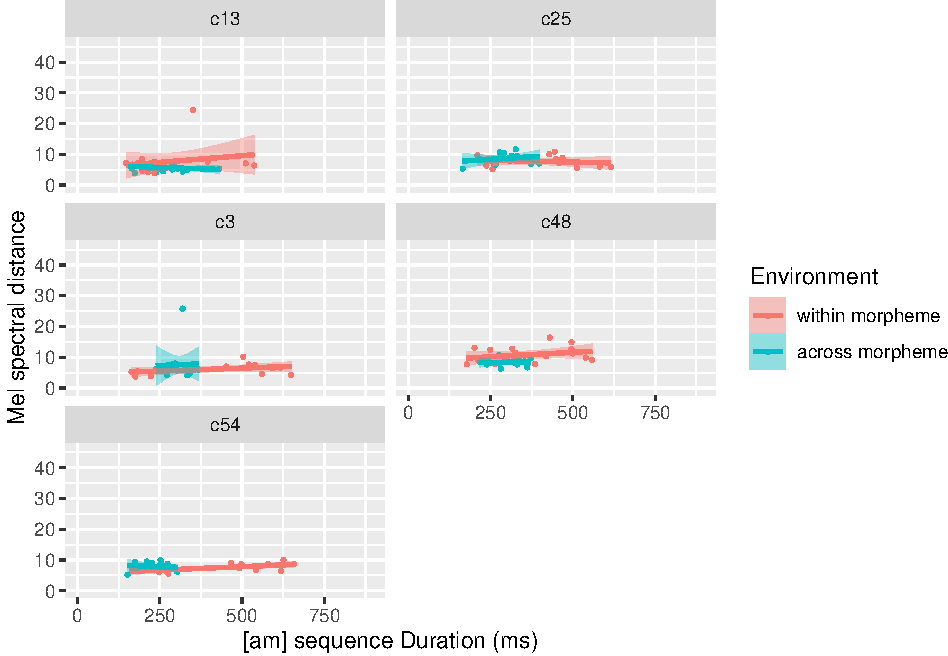
\includegraphics{3_ch3_results_files/figure-latex/nine-facet-am-1.pdf}
\caption{\label{fig:nine-facet-am}Coarticulation by {[}am{]} duration, word, and morphological environment in nine-year-old children}
\end{figure}

\begin{figure}
\centering
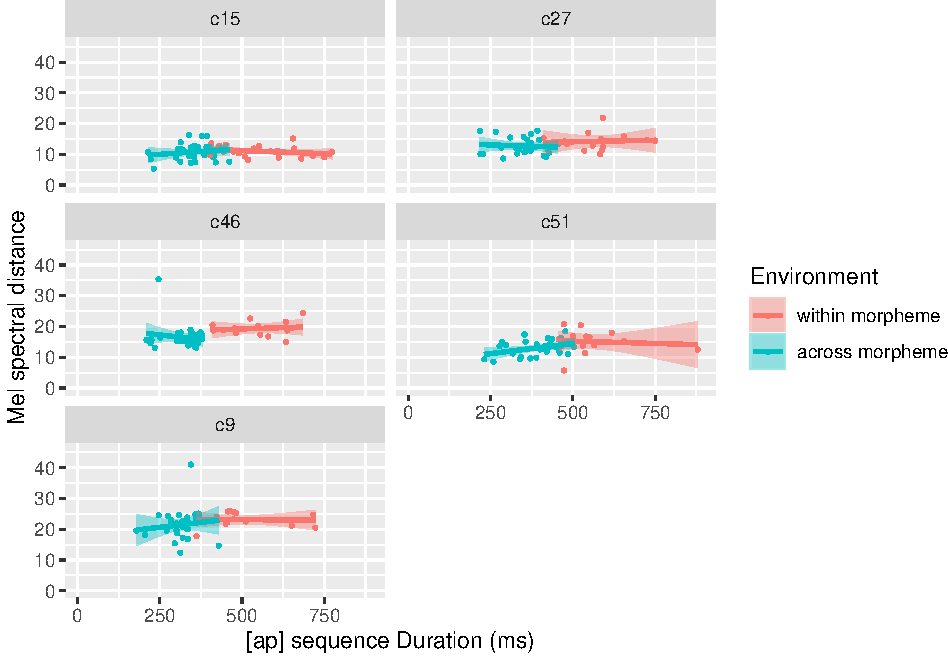
\includegraphics{3_ch3_results_files/figure-latex/ten-facet-ap-1.pdf}
\caption{\label{fig:ten-facet-ap}Coarticulation by {[}ap{]} duration, word, and morphological environment in ten-year-old children}
\end{figure}

\begin{figure}
\centering
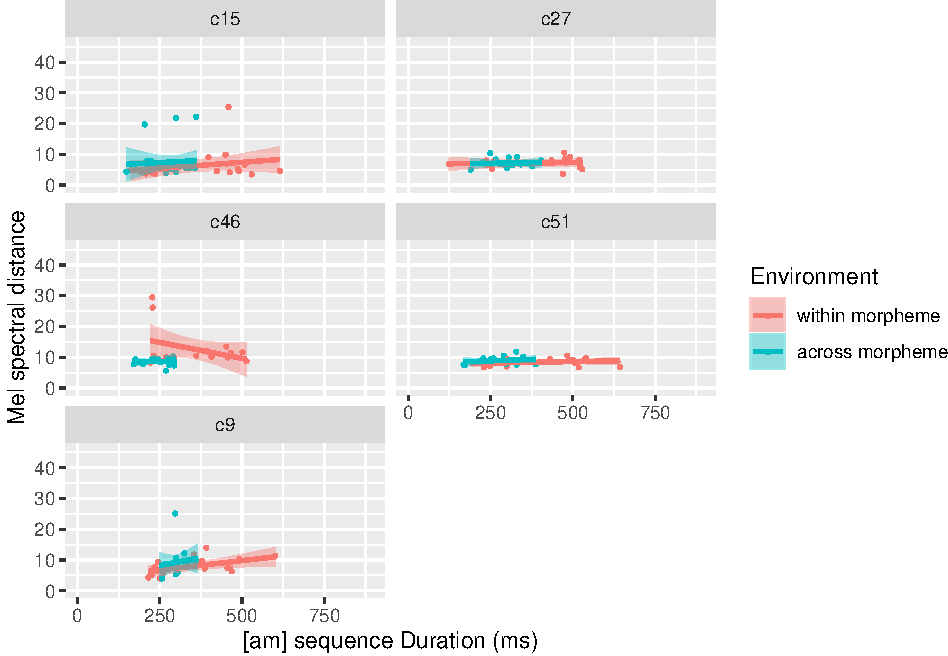
\includegraphics{3_ch3_results_files/figure-latex/ten-facet-am-1.pdf}
\caption{\label{fig:ten-facet-am}Coarticulation by {[}am{]} duration, word, and morphological environment in ten-year-old children}
\end{figure}

\end{document}
